\documentclass[12pt]{article}
\frenchspacing
\usepackage[utf8x]{inputenc}
\usepackage[T2A]{fontenc}
\usepackage{amsmath}
\usepackage{amsfonts}
\usepackage{amssymb}
\usepackage[russian]{babel}
\usepackage{graphicx}
\usepackage{hyperref}
\usepackage{multirow}
\usepackage[left=2cm,right=2cm,top=2cm,bottom=2cm,bindingoffset=0cm]{geometry}
\author{Рашковецкий М.М., группа 526т}
\date{\today}
\title{Лабораторная работа 1.3.3\\Определение вязкости воздуха по скорости течения через тонкие трубки}
\begin{document}
	\maketitle
	
	{\parindent=1cm \hangindent=1cm \parskip=0.5cm
	{\bfseries Цель работы:} экспериментально выявить участок сформированного течения, определить режимы ламинарного и турбулентного течения; определить число Рейнольдса.
	
	\hangindent=1cm
	{\bfseries Оборудование и материалы:} металлические трубки, укреплённые на горизонтальной подставке; газовый счётчик; микроманометр типа ММН; стеклянная U-образная трубка; секундомер.\par}
	
	\section*{Краткая теория}
	
	При малых скоростях течение жидкости является ламинарным (слоистым; скорости частиц направлены по оси трубки), при больших --- турбулентным (слои перемешиваются, скорости частиц в каждой точке быстро меняются и сохраняется только средняя). Критерием, позволяющим определить тип течения, является число Рейнольдса:
	\begin{equation}
	\label{eq:Re}
	\texttt{Re} = \frac{vr \rho}{\eta},
	\end{equation}
	где $v$ --- скорость потока, $r$ --- радиус трубки, $\rho$ --- плотность движущейся среды, $\eta$ --- её вязкость. В гладких трубах круглого сечения переход от ламинарного течения к турбулентному происходит при $\texttt{Re} \approx 1000$.
	
	При ламинарном течении расход определяется формулой Пуазейля:
	\begin{equation}
	\label{eq:puaseile}
	Q=\frac{\pi r^4 \left( P_1 - P_2 \right)}{8l \eta},
	\end{equation}
	где $P_{1,2}$ --- давления в двух выбранных сечениях, $l$ --- расстояние между ними.
	
	Условия применимости формулы \eqref{eq:puaseile}:
	\begin{enumerate}
		\item с запасом выполняется $\texttt{Re} < 1000$;
		\item не происходит заметного изменения плотности газа;
		\item закон распределения скоростей по течению на участке не меняется при движении вдоль потока.
	\end{enumerate}
	
	\begin{figure}[!h]
	\caption{Формирование потока газа в трубке круглого сечения}
	\label{fig:form_str}
	\begin{center}
	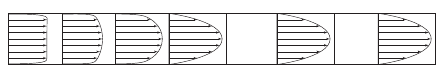
\includegraphics[scale=0.7]{form_str.png}
	\end{center}
	\end{figure}
	
	При втекании газа в трубку из большого резервуара скорости слоёв вначале постоянны по всему сечению (рис. \ref{fig:form_str}), но затем крайние слои тормозятся за счёт стенок трубы и характерное для ламинарного течения параболическое распределение скоростей формируется на расстоянии
	\begin{equation}
	\label{eq:fdist}
	a \approx 0{,}2 r \cdot \texttt{Re}
	\end{equation}
	от начала трубки.
	
	\section*{Экспериментальная установка}
	
	\begin{figure}[!h]
	\caption{Схема установки}
	\label{fig:scheme}
	\begin{center}
	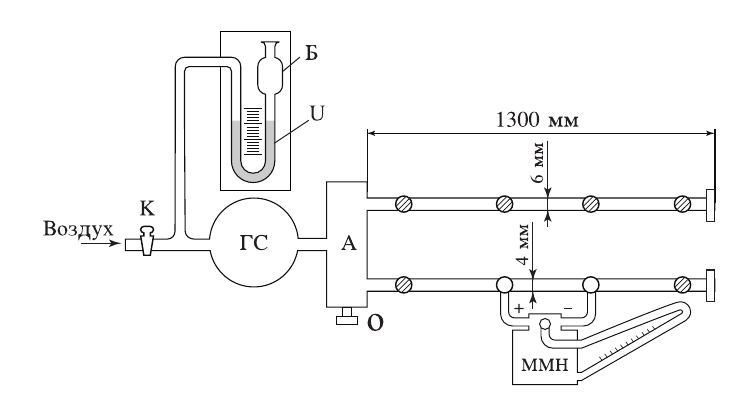
\includegraphics[scale=0.7]{scheme.png}
	\end{center}
	\end{figure}
	
	Схема установки приведена на рис. \ref{fig:scheme}, где:
	\begin{description}
		\item[K] кран для подачи воздуха и регулирования давления;
		\item[ММН] микрометрический манометр;
		\item[ГС] газовый счётчик;
		\item[A] резервуар, к которому припаяны металлические трубки;
		\item[U] U-образная трубка для измерения давления и предохранения газового счётчика (при слишком большом давлении начинает бурлить, привлекая внимание).
		\item[Б] защитный баллон, куда выплёскивается вода при слишком больших перепадах давления.
	\end{description}
	
	Для измерения давления в трубках просверлены миллиметровые отверстия, к двум прикрепляется микроманометр, а другие закрываются пробками.
	
	\begin{figure}[!h]
	\caption{Микрометрический манометр типа ММН}
	\label{fig:mmn}
	\begin{center}
	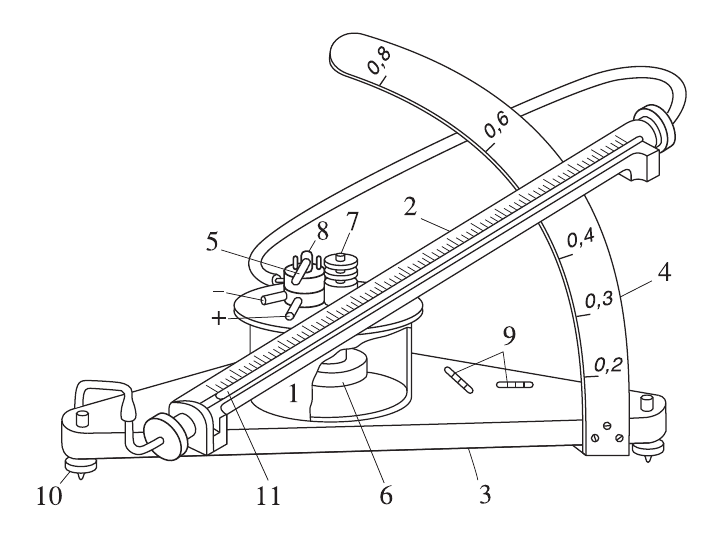
\includegraphics[scale=0.7]{mmn.png}
	\end{center}
	\end{figure}
	
	Микроманометр типа ММН (рис. \ref{fig:mmn}) может измерять перепад давления до 200 мм рт.ст. Он состоит из:
	\begin{enumerate}
		\item цилиндра со спиртом;
		\item трубки со шкалой;
		\item подставки;
		\item стойки с указанными множителями;
		\item рычажка для перевода из режима <<0>> (установка на ноль) в режим <<+>> (измерения);
		\item цилиндр для регулировки нуля;
		\item винта для регулировки глубины погружения цилиндра;
		\item трёхходового крана;
		\item уровни;
		\item регулировочные ножки для установки в горизонтальное положение;
		\item мениска, по которому снимаются показания;
	\end{enumerate}
	
	\begin{figure}[!h]
	\caption{Внешний вид газового счётчика}
	\label{fig:gsout}
	\begin{center}
	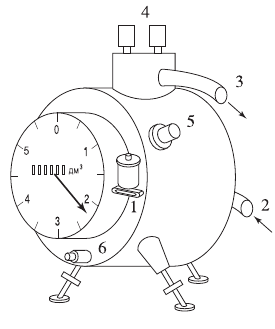
\includegraphics[scale=0.7]{gsout.png}
	\end{center}
	\end{figure}

	Внешний вид газового счётчика показан на рис. \ref{fig:gsout}, где цифрами отмечены:
	\begin{enumerate}
		\item водомерное устройство;
		\item трубка для входа газа; \label{intr}
		\item трубка для выхода газа;
		\item патрубки для присоединения U-образного манометра;
		\item патрубок для установки термометра;
		\item кран для слива воды;
	\end{enumerate}
	
	\begin{figure}[!h]
	\caption{Устройство газового счётчика}
	\label{fig:gsin}
	\begin{center}
	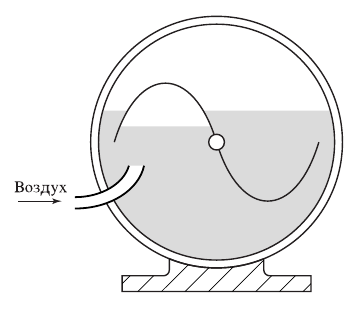
\includegraphics[scale=0.7]{gsin.png}
	\end{center}
	\end{figure}

	Принцип работы счётчика пояснён на рис. \ref{fig:gsin}. На оси вдоль осевой линии цилиндра прикреплены лёгкие чаши. В чашу, находящуюся над трубкой \ref{intr}, поступает воздух. Когда чаша наполняется воздухом, она всплывает и её место занимает следующая. Обороты оси считаются специальным устройством.
	
	\section*{Ход работы}
	
	\begin{enumerate}
		\item Подготовили установку к работе: установили приборы по уровням, проверили наличие воды в газовом счётчике, установили на нуль мениск микроманометра.
		\item Подсоединили микроманометр к последним выводам трубки ($d = \left(3{,}90\pm 0{,}05 \right)$ мм) на участке со сформировавшимся потоком (к последним двум отверстиям, т.к. согласно \eqref{eq:fdist} $a \approx 40$ см, расстояние между ними $l=50$ см), открыли эту трубку.
		\item Медленно открывая кран K и впуская воздух в установку, внимательно следили за показаниями манометра.
		\item Сняли зависимость $\Delta P$ от $Q=\Delta V /\Delta t$, где $\Delta V$ измеряли газовым счётчиком, а $\Delta t$ --- секундомером, во всём доступном диапазоне перепадов давлений.
		\item При расходе, обеспечивающем ламинарность течения, измерили распределение давления вдоль трубки, измерив перепад давлений по всем парам отверстий.
	\end{enumerate}
	
	\section*{Обработка результатов}
	
	В таблице \ref{tbl:res_p_q} приведены результаты измерений зависимости $\Delta P$ от $Q$.
	
	\begin{table}[!h]
		\caption{Результаты измерений $\Delta P$ от $Q$}
		\label{tbl:res_p_q}
		\begin{center}
		\begin{tabular}{|c|c|c|c|c|c|}
			\hline
			$\Delta h$, см & $K$ & $\Delta V$, л & $\Delta t$, с & $\Delta P$, Па & $Q, \text{см}^3/\text{с}$ \\
			\hline
			1,85 & 0,2 & 1,5 & 66 & $29{,}4\pm 0{,}8$ & $22{,}7\pm 0{,}2$ \\
			0,85 & 0,2 & 0,5 & 50 & $13{,}5\pm 0{,}8$ & $10{,}0\pm 0{,}1$ \\
			3,4 & 0,2 & 1,5 & 37 & $54{,}0\pm 0{,}8$ & $40{,}5\pm 0{,}5$ \\
			4,6 & 0,2 & 2,5 & 44 & $73{,}0\pm 0{,}8$ & $56{,}8\pm 0{,}6$ \\
			5,7 & 0,2 & 3 & 43 & $90{,}5\pm 0{,}8$ & $69{,}8\pm 0{,}8$ \\
			7,3 & 0,2 & 3 & 34 & $115{,}9\pm 0{,}8$ & $88{,}2\pm 1{,}3$ \\
			9,1 & 0,2 & 4 & 42 & $144{,}5\pm 0{,}8$ & $95{,}2\pm 1{,}1$ \\
			12,1 & 0,2 & 4 & 39 & $192{,}1\pm 0{,}8$ & $102{,}6\pm 1{,}3$ \\
			17,7 & 0,2 & 5 & 41 & $281{,}0\pm 0{,}8$ & $122{,}0\pm 1{,}5$ \\
			24,7 & 0,2 & 5,5 & 38 & $392{,}2\pm 0{,}8$ & $144{,}7\pm 1{,}9$ \\
			27,3 & 0,2 & 7 & 45 & $433{,}4\pm 0{,}8$ & $155{,}6\pm 1{,}7$ \\
			20,6 & 0,2 & 5,5 & 41 & $327{,}1\pm 0{,}8$ & $134{,}1\pm 1{,}6$ \\
			15,2 & 0,2 & 5 & 43 & $241{,}3\pm 0{,}8$ & $116{,}3\pm 1{,}4$ \\
			15,2 & 0,4 & 7,5 & 45 & $482{,}7\pm 1{,}6$ & $166{,}7\pm 1{,}9$ \\
			18,2 & 0,4 & 7,5 & 41 & $577{,}9\pm 1{,}6$ & $183\pm 2$ \\
			21,0 & 0,4 & 10 & 51 & $666{,}8\pm 1{,}6$ & $196{,}1\pm 1{,}9$ \\
			24,1 & 0,4 & 12 & 57 & $765{,}3\pm 1{,}6$ & $210{,}5\pm 1{,}8$ \\
			\hline
		\end{tabular}
		\end{center}
	\end{table}
	
	Давление посчитано по формуле
	$$ \Delta P = K\rho g \Delta h. $$
	
	Погрешности оценены из таких соображений: $\sigma_{\Delta h}=0{,}05$ см $\Rightarrow \sigma_{\Delta P}=K \rho \sigma_{\Delta h}$; объём фиксировался по делениям, поэтому его измерение считаем точным, а вот $\sigma_{\Delta t}=0{,}5$ с, поэтому $\sigma_Q=Q \frac{\sigma_{\Delta t}}{\Delta t}$.
	
	\begin{figure}[!h]
	\caption{График зависимости перепада давлений от расхода}
	\label{fig:graph_p_q}
	\begin{center}
	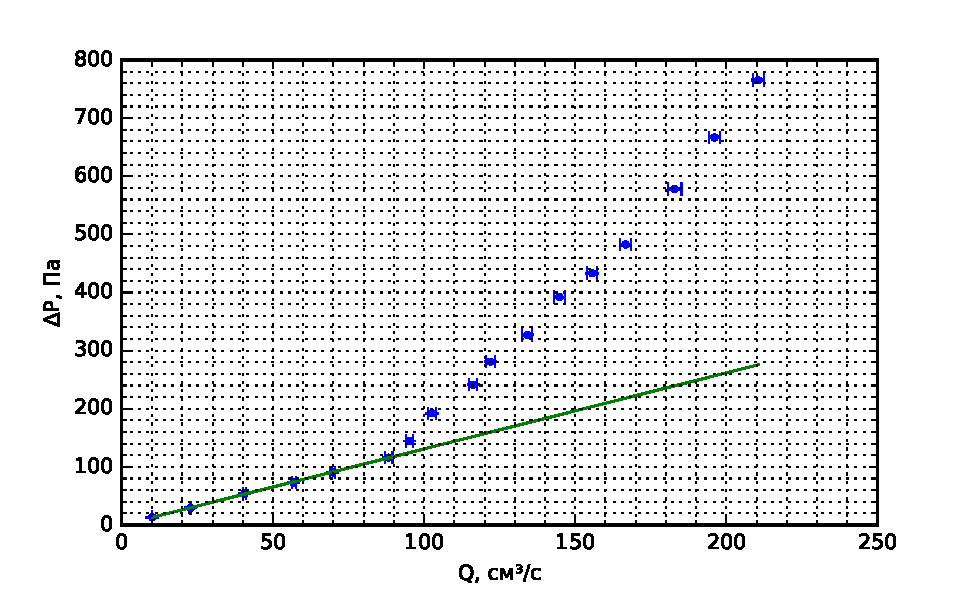
\includegraphics[scale=1]{graph_p_q.pdf}
	\end{center}
	\end{figure}
	
	По этим данным был построен график (рис. \ref{fig:graph_p_q}). Видно, что первые 6 точек хорошо ложатся на прямую, а дальше график начинает заметно отклоняться от прямолинейного. Эти 6 точек были аппроксимированы прямой по МНК с учётом весов точек по формуле $$ Q = k \Delta P. $$
	Эта прямая также нанесена на график.
	
	Согласно \eqref{eq:puaseile}, вязкость через угловой коэффициент выражается как
	\begin{equation}
		\label{eq:visc_from_k}
		\eta = \frac{\pi r^4}{8l k}.
	\end{equation}
	Соответственно, погрешность равна $$ \sigma_\eta = \eta \sqrt{\left( \frac{\sigma_k}{k} \right)^2 + \left( 4 \frac{\sigma_r}{r} \right)^2} $$
	
	Получены результаты: $$ k = \left( 7{,}64\pm 0{,}06 \right) \cdot 10^{-7} \frac{\text{Па} \cdot \text{с}}{\text{м}^3}, $$
	$$ \eta = \left( 14{,}9\pm 0{,}8 \right) \,\text{мкПа} \cdot \text{с}. $$
	
	В справочнике (Енохович А.С. Краткий справочник по физике. М., <<Высш. школа>>, 1976) приведена вязкость воздуха при температуре $t_1=20^\circ \text{C}$ $\eta_1 = 18{,}1 \,\text{мкПа} \cdot \text{с}$, а при $t_2=100^\circ \text{C}$ --- $\eta_2 = 21{,}2 \,\text{мкПа} \cdot \text{с}$. Наш результат получился заниженным значительно больше погрешности, возможно, это объясняется некоторыми отличиями в составе воздухе, например, большей влажностью (водяной пар имеет меньшую вязкость в этом диапазоне температур).
	
	Переходной областью от ламинарного к турбулентному течению условно можно считать 7--11 точки, для них числа Рейнольдса $$\texttt{Re}_7\approx 1350,$$ $$\texttt{Re}_{11}\approx 1900,$$ принимая $\rho \approx 1,3 \frac{\text{кг}}{\text{м}^3}$. Переход наблюдается даже несколько позже, чем предсказывала теория.
	
	Затем около третьей точки (по расходу, $\texttt{Re}_3\approx 500$) приведены разности давлений между всеми парами доступных отверстий (таблица \ref{tbl:res_p_l}). Они аддитивны в пределах погрешности ($\sigma_{\Delta h}=0{,}05$ см). Расстояния между соседними отверстиями: $l_{01}=11{,}5$ см, $l_{12}=30$ см, $l_{23}=40$ см, $l_{34}=50$ см.
	
	\begin{table}[!h]
		\caption{Разность давлений для пар отверстий}
		\label{tbl:res_p_l}
		\begin{center}
		\begin{tabular}{|c|ccccc|}
			\hline
			$\Delta h_{ij}$, см & 0 & 1 & 2 & 3 & 4 \\
			\hline
			0 & -- & 3,7 & 10,2 & 14,7 & 20,1 \\
			1 & 3,7 & -- & 6,5 & 11,0 & 16,5 \\
			2 & 10,2 & 6,5 & -- & 4,5 & 10,0 \\
			3 & 14,7 & 11,0 & 4,5 & -- & 5,5 \\
			4 & 20,1 & 16,5 & 10,0 & 5,5 & -- \\
			\hline
		\end{tabular}
		\end{center}
	\end{table}
	
	По этим данным был построен график $\Delta h_{i4} \left( l_{i4} \right)$ (рис. \ref{fig:graph_p_l}).
	
	\begin{figure}[!h]
	\caption{График зависимости перепада давлений от расстояния}
	\label{fig:graph_p_l}
	\begin{center}
	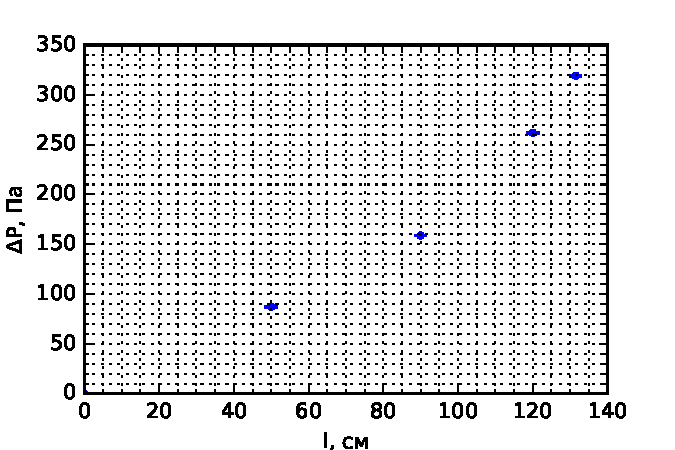
\includegraphics[scale=1]{graph_p_l.pdf}
	\end{center}
	\end{figure}
	
	Поскольку точек мало, судить о линейности и соответственно ламинарности достаточно сложно, но первые (от нуля) три точки почти ложатся на прямую, т.е. формирование потока завершается около второго отверстия и экспериментальное значение $a*\approx 40$ см, как и предсказано по \eqref{eq:fdist}.
	
\end{document}
